\chapter{Grundlagen}

\section{Einführung in cFront}
\textit{cFront} ist eine Anwendung, welche von der Abteilung cGroup Solutions innerhalb der \ac{LSY} entwickelt wird. Es handelt sich bei der Anwendung um ein Tool, welches an Flughafen Terminals eingesetzt wird. 

Es agiert dabei als Interface für mehrere Anwendung und ermöglicht es dem Nutzer, diese Anwendungen zu starten. Welche Anwendungen sichtbar sind, können je nach Kunde individuell konfiguriert werden. 
\begin{figure}[h]
	\centering 
	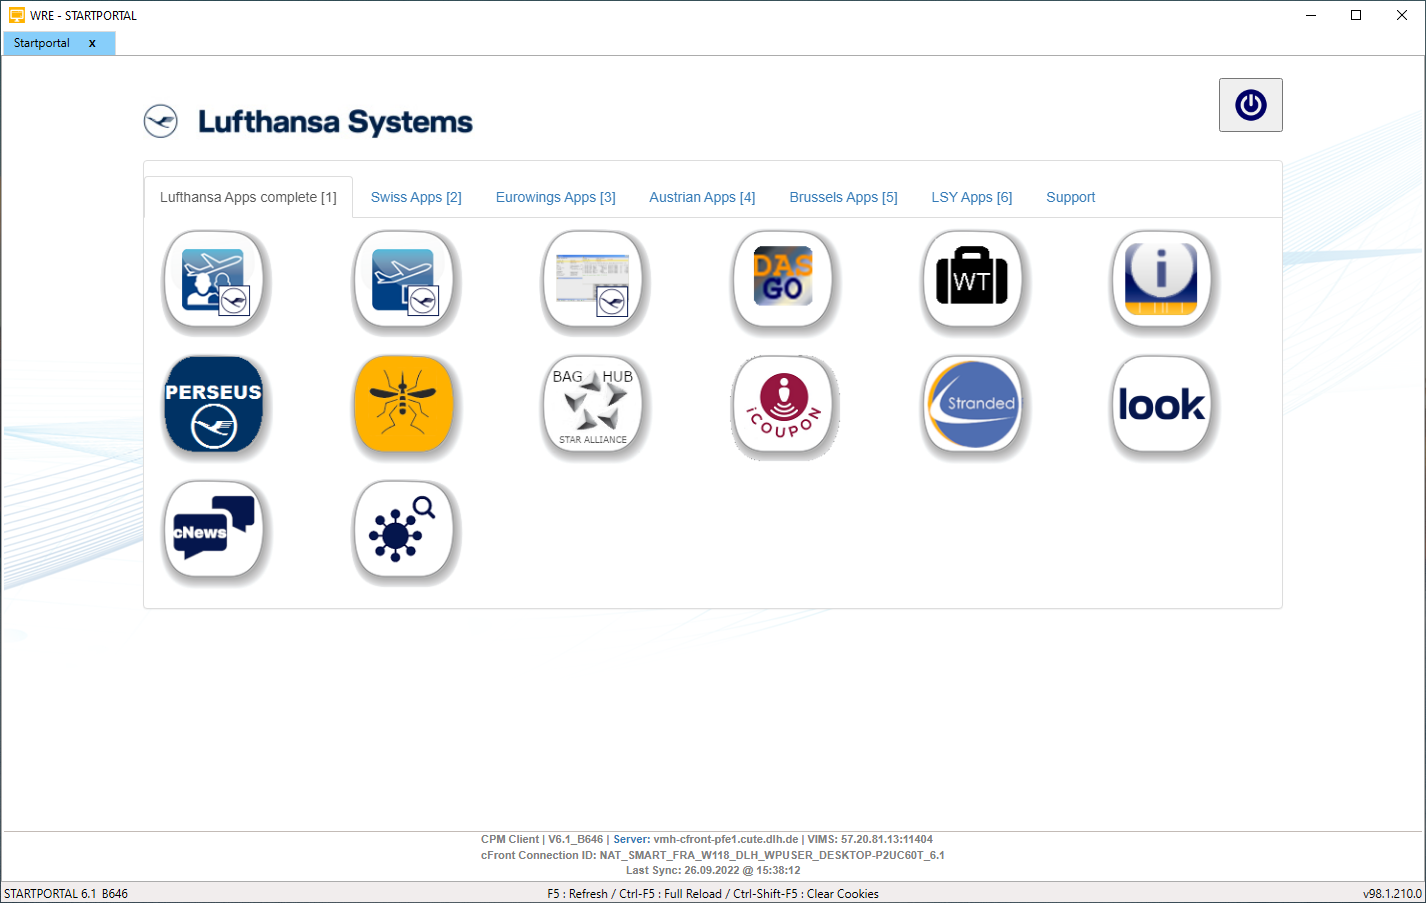
\includegraphics[width=1\textwidth]{img/abbildungen/MicrosoftTeams-image (3).png}
	\captionsetup{format=hang}
	\caption{Umsetzungsmöglichkeit mit Keycloak}
\end{figure}

\section{CIA-Triade}

Die CIA-Triade gehört zu den wichtigsten Darstellungen von Sicherheitszielen innerhalb der Informationssicherheit. Sie beschreibt die drei Schutzziele \textit{Confidentiality} (Vertraulichkeit), \textit{Integrity} (Integrität) und \textit{Availability} (Verfügbarkeit). Im Folgenden werden diese kurz beschrieben:

\begin{figure}[h]
	\centering 
	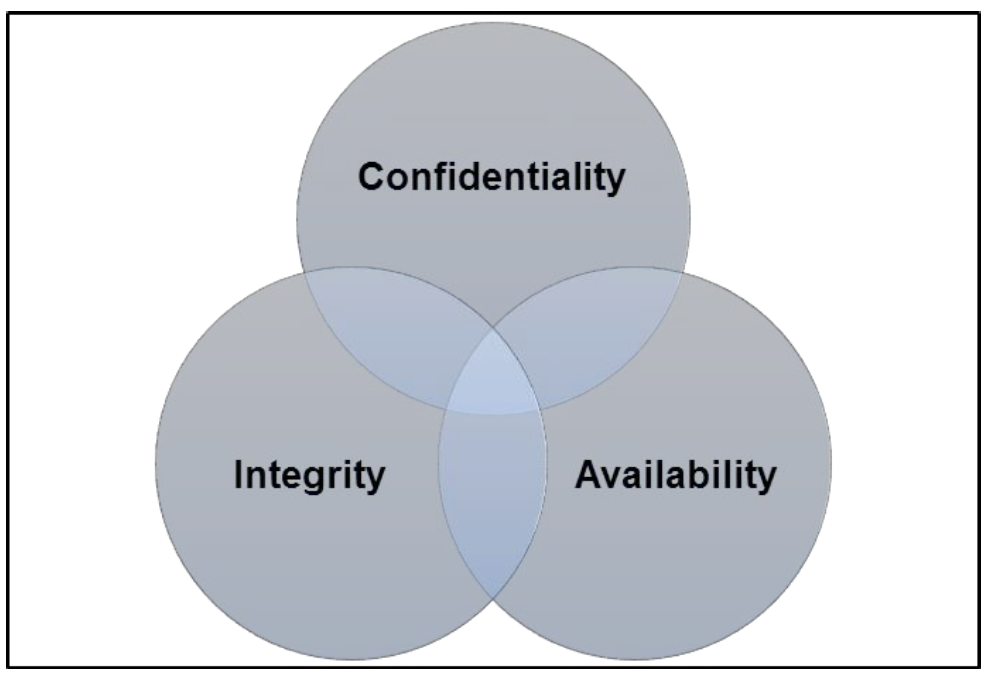
\includegraphics[width=0.5
    \textwidth]{img/abbildungen/CIA-Triad.png}
	\captionsetup{format=hang}
	\caption{Umsetzungsmöglichkeit mit Keycloak}
\end{figure}

\begin{figure}[h]
	\centering 
	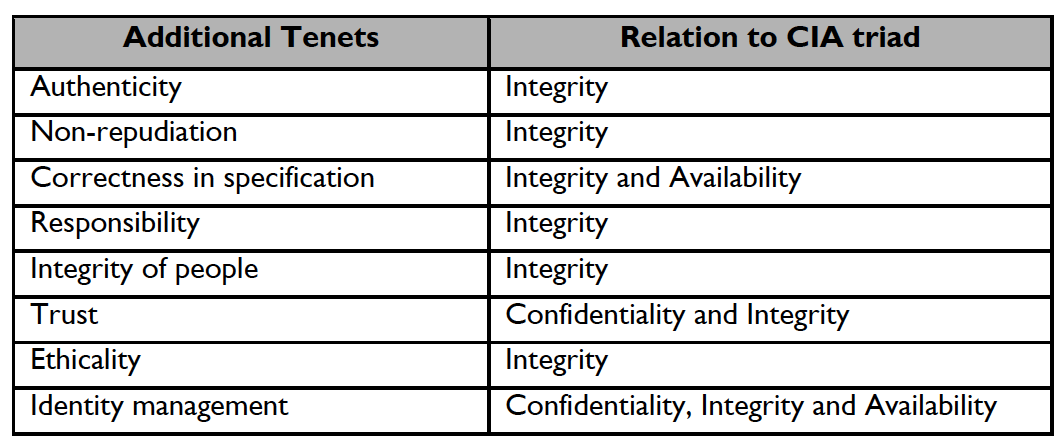
\includegraphics[width=0.8\textwidth]{img/abbildungen/Schutzziele.png}
	\captionsetup{format=hang}
	\caption{Umsetzungsmöglichkeit mit Keycloak}
\end{figure}

\begin{itemize}
    \item Vertraulichkeit gehört zu den wichtigsten Schutzzielen in der Informationssicherheit \cite{samonas2014cia}.
    \item Kommt vom lateinischen Wort \textit{confidere} \cite{samonas2014cia}.
    \item besagt, dass Informationen und Daten geschützt werden müssen, sodass diese nur von autorisierten Personen und für autorisierte Zwecke genutzt werden können \cite{samonas2014cia}.
    \item Einschränkungen des Zugriffs auf Informationen und Daten, um die Privatssphäre und persönliches Eigentum zu schützen \cite{samonas2014cia}.
    \item Da der Fokus immer mehr auf wirtschaftliche Aspekte liegt, hat die Vertraulichkeit im Vergleich zu früher an Bedeutung verloren \cite{samonas2014cia}.
    \item Wird beispielsweise geschützt durch Verschlüsselung, Authentifizierung oder Sicherheitsprotokolle \cite{agarwal2011security}.
    \item kommt vom lateinischen \textit{tangere}, was so viel wie berühren bedeutet. Mit der Vorsilbe \textit{In-} wird daraus etwas, was so viel bedeutet wie \textit{unberührbar} \cite{samonas2014cia}.
    \item Beinhaltet die Garantie, dass Daten nicht verändert werden können, ohne dass dies bemerkt wird \cite{agarwal2011security}.
    \item Beispielsweis, dass eine empfangene Nachricht genau so ankommt, wie sie gesendet wurde \cite{agarwal2011security}.
    \item Wird beispielsweise geschützt durch Firewall, Intrusion Detection Systeme oder digitale Signaturen \cite{agarwal2011security}.
    \item kommt vom lateinischen \textit{valere} was so viel bedeutet wie \textit{stark sein} \cite{samonas2014cia}.
    \item In der Informationssicherheit bezieht sich die Zuverlässigkeit auf einen zeitnahen und zuverlässigen Zugriff auf Informationen und Daten \cite{samonas2014cia}.
    \item Das bedeutet dass der Zugriff möglichst ohne unterbrechungen und unabhängig vom Standort erreichbar werden kann \cite{agarwal2011security}. 
    \item Verfügbarkeit kann beispielsweise durch Netzwerksicherheit oder Fehlertoleranz (beispielsweise bein Authentifizierungsversuche) gewährleistet werden \cite{agarwal2011security}.
\end{itemize}

\section{Arten der Authentifizierung}

\begin{figure}[h]
	\centering 
	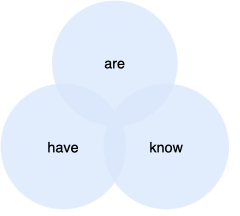
\includegraphics[width=0.4\textwidth]{img/abbildungen/factors.png}
	\captionsetup{format=hang}
	\caption{Umsetzungsmöglichkeit mit Keycloak}
\end{figure}

\begin{itemize}
    \item Die Authentifizierung dient häufig als erste Verteidigungslinie von Systemen. \cite{boonkrong2012security}
    \item Faktor Something you know. Diese Methode nutzt Informationen, welche nur dem Nutzer bekannt sind, um seine Identität zu bestätigen \cite{boonkrong2012security}.
    \item Faktor Something you have. Diese Methode nutzt physische Objekte, welche sich im Besitz des Nutzers befinden, um seine Identität zu bestätigen. Dazu gehören u.a. Smartcards und Hardware-Token \cite{boonkrong2012security}.
    \item Faktor Something you are. Diese Methode nutzt biometrische Daten des Nutzers, um seine Identität zu bestätigen. Dazu gehören u.a. Fingerabdrücke, Iris-Scans und Gesichtserkennung \cite{boonkrong2012security}.
    \item Ein Problem dieser Methode ist, dass sich menschliche Eigenschaften im Laufe der Zeit verändern können. Auch Verletzungen oder Krankheiten können die biometrischen Daten verändern \cite{boonkrong2012security}.
    \item Nicht standardmäßig, aber weiterer Faktor ist something you perform or produce. Diese Methode nutzt beispielsweise die Stimme oder die (digitale) Unterschrift des Nutzers, um seine Identität zu bestätigen \cite{boonkrong2012security}.
\end{itemize}


\section{Passwortbasierte Authentifizierung}\label{pw-auth}

\begin{figure}[h]
	\centering 
	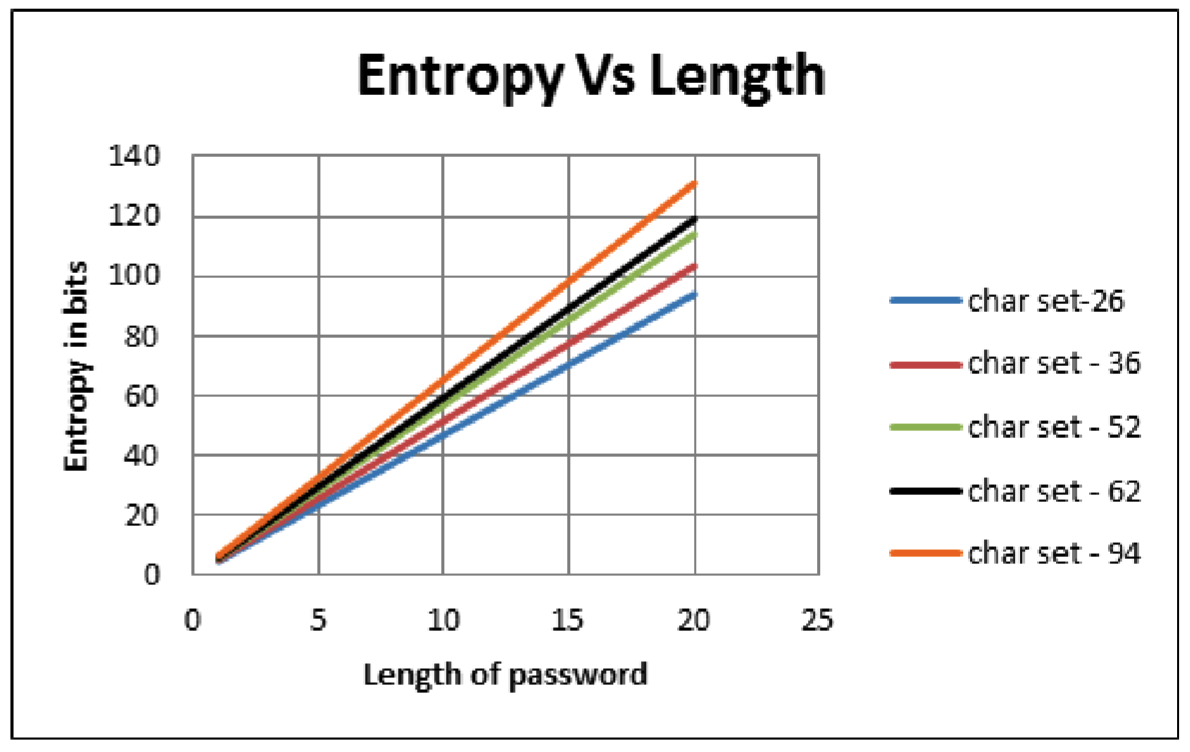
\includegraphics[width=0.7\textwidth]{img/abbildungen/entropy-length.png}
	\captionsetup{format=hang}
	\caption{Umsetzungsmöglichkeit mit Keycloak}
\end{figure}

\begin{figure}[h]
	\centering 
	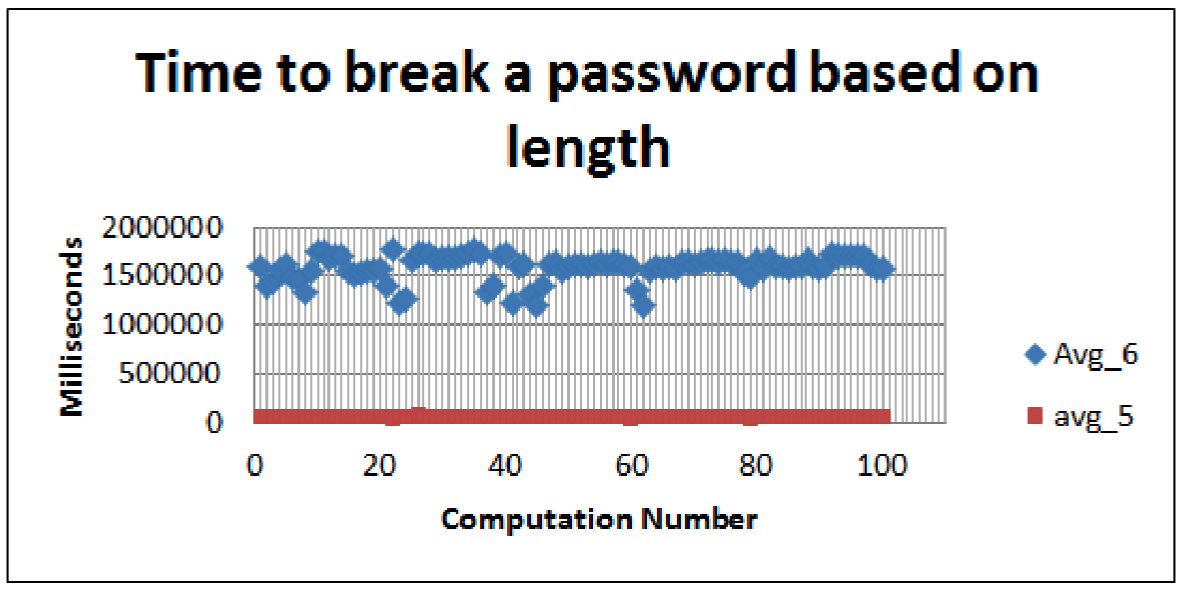
\includegraphics[width=0.7\textwidth]{img/abbildungen/length-time.png}
	\captionsetup{format=hang}
	\caption{Umsetzungsmöglichkeit mit Keycloak}
\end{figure}

\begin{itemize}
    \item Die heutzutage am häufigsten genutzte Methode zur Authentifizierung ist die passwortbasierte Authentifizierung \cite{chanda2016password} \cite{boonkrong2012security} \cite{yildirim2019encouraging}.
    \item Die Sicherheit von Systemen basiert somit auf der Sicherheit der Passwörter \cite{boonkrong2012security}.
    \item Passwörter gelten als eins der größten Risiken für Systeme, da sie viele Angriffsvektoren bieten \cite{yildirim2019encouraging} \cite{farke2020you}.
    \item 81\% der Hackerangriffe basierten auf der Kompromittierung von Passwörtern \cite{barbosa2021provable}. 
    \item 2017 waren Phishing E-Mails die häufigste Angriffsmethode \cite{barbosa2021provable}.
    \item Obwohl es bereits alternative Ansätze gibt, werden Passwörter weiterhin genutzt. Das liegt an der Einfachheit und dem geringen Aufwand, welche die Nutzung von Passwörtern mit sich bringt \cite{yildirim2019encouraging}.
    \item Eine Vielzahl an großen Unternehmen wurden bereits Opfer von der Veröffentlichung von Passwörtern, obwohl ein hoher Aufwand betrieben wird diese zu schützen. Da sich die Enthüllung der Passwörter allerdings als Angriffsziel bei Angreifern etabliert hat, ist selbst ein hoher Aufwand nicht ausreichend \cite{boonkrong2012security}.
    \item Dabei handelt es sich am häufigsten um alphanumerische Passwörter, welche aus einer Kombination von Groß- und Kleinbuchstaben, Zahlen und Sonderzeichen bestehen \cite{chanda2016password}. 
    \item Passwörter können durch verschiedene Angriffe kompromittiert werden. Angreifer können Zugriff auf die Datenbank erhalten, in welcher die Passwörter gespeichert sind. Aber auch auf persönlicher Ebene können Passwörter erlangt werden. Aufgeschriebene Passwörter können in fremde Hände geraten. Auch Social Engineering kann genutzt werden, um Passörter mit Hilfe von Phishing oder Keyloggern zu erlangen. Häufig lassen sich Passwörter allerdings auch mit Hilfe von Brute-Force- oder Dictionary-Attacken kompromittieren \cite{chanda2016password} \cite{morii2017research}.
    \item Brute-Force-Attacken versuchen alle möglichen Kombinationen von Zeichen, welche ein Passwort enthalten kann, auszuprobieren. Je höher dabei die Anzahl an möglichen Kombinationen ist, desto aufwändiger wird es ein Passwort zu erraten.
    \item Je länger ein Passwort, desto schwieriger zu knacken. Länge auch wichtiger als Zeichenraum \cite{chanda2016password}.
    \item Hier auch kurz auf die Mathematik dahinter eingehen.
    \item Studien zeigen, dass Nutzer dazu neigen gleiche oder ähnliche Passwörter für verschiedene Zugänge zu nutzen \cite{chanda2016password} \cites{ives2004domino}.
    \item Verfügen Angreifer über ein Passwort eines Nutzers, können häufig auch andere Zugänge übernommen werden \cite{chanda2016password} \cite{morii2017research}.
    \item Obwohl die Angriffsvektoren und Schwachstellen von Passwörtern schon lange bekannt sind, bleiben diese unverändert bestehen. \cite{ives2004domino}.
\end{itemize}

\subsection{Speicherung}

\begin{itemize}
    \item Viele Angreifer versuchen Passwörter zu kompromittieren, indem sie Zugriff auf die Datenbank erhalten, in welcher die Passwörter gespeichert sind. Mit Hilfe von Passwörtern erhoffen sich die Angreifer Zugriff auf Systeme und Netzwerke \cite{boonkrong2012security}.
    \item Passwörter können auf verschiedene Arten gespeichert werden. Dadurch können verschiedene Angriffsvektoren entstehen \cite{chanda2016password}.
    \item Plaintext am schlechtesten. Werden die Passwörter in lesbarer Form gespeichert, können Angreifer alle Passwörter auslesen, sobald sie Zugriff auf die Datenbank haben. Dabei muss kein weiterer Aufwand betrieben werden \cite{chanda2016password}.
    \item Verschlüssellung besser, aber nicht optimal. Verschlüssellung ist zurückführbar. Gelangen Angreifer an den benötigten Schlüssel, können sie alle Passwörter entschlüsseln und auslesen \cite{chanda2016password}.
    \item AM besten Hashing mit Salt. Sobald ein Passwort gehasht wurde, kann es nicht mehr zurückgerechnet werden. Durch einen individuellen Salt kann ebenfalls verhindert werden, dass Angreifer die Passwörter mit Hilfe von Rainbow-Tables entschlüsseln können \cite{chanda2016password}.
    \item auch noch zwei salts möglich - einer public einer private. schützt vor offline angriffen \cite{chanda2016password}.
    \item Vielleicht hier noch ganz kurz auf Hash Funktionen eingehen?
\end{itemize}

\subsection{Faktor Mensch}

\begin{itemize}
    \item Die Sicherheit ist nicht nur von den technischen Aspekten abhängig \cite{ives2004domino}.
    \item Ein Großteil der Angriffsfläche von Passwörtern entsteht durch den Faktor Mensch \cite{yildirim2019encouraging}.
    \item Von Menschen erstellte Passwörter sind keine echten Zufallswerte. Das liegt insbesondere daran, dass Nutzer sich Passwörter merken können müssen. Daher beinhalten Passwörter häufig Informationen, welche einen Bezug zum Nutzer haben. Dazu gehören beispielsweise Namen, Geburtsdaten, Adressen oder andere persönliche Informationen. Auch Passwörter, welche einfache Tastaturmuster beinhalten sind sehr beliebt. Dazu zählen beispielsweise \glqq qwertz\grqq{} oder \glqq 123456\grqq{} \cite{chanda2016password} \cite{boonkrong2012security} \cite{yildirim2019encouraging}.
    \item Das Hauptproblem entsteht dabei durch die benötigte Einprägsamkeit der Passwörter \cite{yildirim2019encouraging}.
    \item Es ist sehr schwierig für Nutzer sich verschiedene komplexe Passwörter zu merken. Daher neigen Nutzer dazu, einfache Passwörter zu nutzen oder Passwörter für verschiedene Zugänge zu wiederholen \cite{chanda2016password}.
    \item Das ist der Hauptgrund dafür, dass Nutzer dazu neigen, einfache Passwörter zu nutzen oder Passwörter für verschiedene Zugänge zu wiederholen \cite{yildirim2019encouraging}.
    \item Diese Faktoren führen dazu dass die Anzahl an genutzten Passwörtern deutlich geringer ist als die gesamte Menge an möglichen Passwörtern \cite{boonkrong2012security}.
    \item Ebenfalls ist häufig die Motivation der Nutzer gering komplexe Passwörter zu erstellen. Dies liegt häufig daran, dass die Nutzer nicht die Gefahr erkennen und nicht überzeugt von Guidelines und Richtlinien zur Erstellung von Passwörtern sind \cite{yildirim2019encouraging}.
    \item Nutzer tendieren dazu bewusst schwache Passwörter zu erstellen, die den Anforderungen der Richtlinien entsprechen. Das führt zu einem kontraproduktiven Effekt, da die Sicherheit geringer wird \cite{yildirim2019encouraging}.
    \item Sehr komplexe Richtlinien führen demnach nicht zwangsmäßig zu einer höheren Sicherheit. Vielmehr kann das Gegenteil erreicht werden \cite{yildirim2019encouraging} \cite{morii2017research}.
    \item Aktive Internet-Nutzer verwalten durchschnittlich 15 Passwörter pro Tag \cite{ives2004domino}.
    \item Eine der größten Schwachstellen ist also die Wahl des Passwortes durch den Nutzer \cite{boonkrong2012security}.
    \item Ein Domino Effekt kann entstehen, wenn mit Hilfe eines Passwortes weitere Passwörter kompromittiert werden. So können mehrere Systeme indirekt davon betroffen sein, sobald ein Passwort kompromittiert wurde \cite{ives2004domino}.
    \item Das macht von Menschen erstellte Passwörter anfälliger für Angriffe, da diese einfacher zu erraten sind \cite{chanda2016password}.
    \item 
\end{itemize}

\section{Passwortlose Authentifizierung}

\begin{itemize}
    \item Unter der passwortlosen Authentifizierung werden verschiedene Verfahren zusammengefasst, welche die Nutzung von Passwörtern ersetzen.
    \item Während bei passwortbasierten Verfahren also der Faktor \textit{something you know} genutzt wird, wird bei passwortlosen Verfahren auf andere Faktoren zurückgegriffen.
    \item Die \ac{FIDO} Allianz nutzt die Bezeichnung passwortlos, um eine \ac{SFA} oder \ac{MFA} mit Hilfe eines Authentifizierungsgerätes zu beschreiben \cite{farke2020you}.
    \item Passwortlose Verfahren werden als sicherer angesehen, da viele der in \textbf{\nameref{pw-auth}} aufgeführten Angriffsvektoren nicht auf passwortlose Ansätze anwendbar sind \cite{chowhan2019password} \cite{parmar2022comprehensive}.
    \item Auch die Benutzerfreundlichkeit soll durch passwortlose Verfahren verbessert werden, da diese sich keine Passwörter mehr merken müssen \cite{chowhan2019password}.
    \item Allerdings haben sich passwortlose Verfahren noch nicht durchgesetzt und sind nicht weit verbreitet.
    \item Das liegt auch daran, dass für passwortlose Verfahren häufig zusätzliche Hardware benötigt wird, welche mit zusätzlichen Kosten verbunden ist \cite{chowhan2019password}.
    \item Auch die Umgewöhnung an eine neue Art der Authentifizierung wird als eine Hürde für die Etabliserung von passwortlosen Verfahren angesehen \cite{chowhan2019password}.
    \item Viele verschieden Möglichkeiten Passswortlose Authentifizierung zu implementieren:
    \item lediglich ein Überblick, da eine detailiertere BEschreibung den Scope dieser Arbeit überschreiten würde.
\end{itemize}

\begin{figure}[h]
	\centering 
	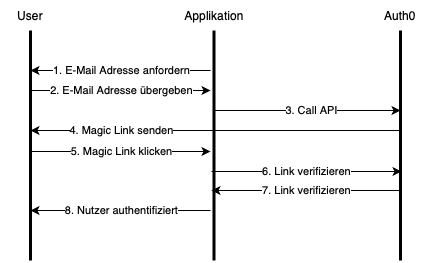
\includegraphics[width=0.7\textwidth]{img/abbildungen/magic_link.png}
	\captionsetup{format=hang}
	\caption{Umsetzungsmöglichkeit mit Keycloak}
\end{figure}

\begin{itemize}
    \item Magic Link:
    Bei einem Magic Link handelt es sich um eine
    Authentifizierungsmöglichkeit, bei welcher Nutzer
    lediglich ihren Benutzernamen oder ihre E-Mail-Adresse
    zur Anmeldung angeben müssen. Anschließend erhält der Nutzer eine E-Mail mit einem dazugehörigen Link, welcher genutzt wird, um seine Identität zu bestätigen. \cite{chowhan2019password} \cite{parmar2022comprehensive}
    Dieser Link beinhaltet einen Authentication Code, welcher im Hintergrund abgeglichen und validiert wird. Ist die Validierung erfolgreich wird der Nutzer authentifiziert und angemeldet. Nach der Anmeldung verliert der AUthentication Code seine Gültigkeit und somit auch der Link selbst. \cite{chowhan2019password}
    Die Sicherheit dieses Verfahrens basiert dabei auf der Annahme, dass der Mail-Server bzw. der Zugang zum Account des Nutzers ausreichend geschützt ist. Ist diese Annahme nicht gegeben können sich auch andere Personen mit dem Link des eigentlichen Nutzers authentifizieren ohne autorisiert zu sein. \cite{chowhan2019password}
    Passwort bleibt für Zugriff auf E-Mail Zugang notwendig, allerdings würde so die Anzahl an Passwörtern für den Nutzer reduziert werden.
    Vorteile:
    Sehr benutzerfreundlich und einfach \cite{parmar2022comprehensive}.
    Implementierung und Kosten zur Instandshaltung verhältnißmäßig gering \cite{parmar2022comprehensive}.
    Nachteile:
    Nutzung von Spam-Filtern, kann die Benutzerfreundlichkeit stark beeinträchtigen. So könnten die zugehörigen Mails fälschlicherweise als Spam klassifiziert werden oder eine erhöhte Wartezeit auf die Mail entstehen \cite{parmar2022comprehensive}.
    Die Sicherheit des Verfahrens hängt von der Sicherheit des Mail-Servers ab. Ist dieser nicht ausreichend geschützt, können Angreifer Zugriff auf die Mails erhalten und sich somit auch mit dem Link authentifizieren \cite{chowhan2019password}.
    Dies kann geschehen, ohne dass der Nutzer davon etwas mitbekommt \cite{chowhan2019password}.
    \item \ac{OTP}:
    Das Konzept hinter \ac{OTP}s ähnelt dem des Magic Links. Nutzer geben ihre E-Mail-Adresse oder ihre Handynummer an (diese können ebenfalls einem Benutzernamen zugewiesen sein) und erhalten eine E-Mail/SMS, welche ein \ac{OTP} beinhaltet \cite{chowhan2019password} \cite{parmar2022comprehensive}. 
    Dieses Wird vom System abgeglichen und validiert. Ist die Validierung erfolgreich wird der Nutzer authentifiziert und angemeldet. Nach der Anmeldung verliert das \ac{OTP} seine Gültigkeit. \cite{chowhan2019password}
    Häufig werden \ac{OTP}s allerdings nicht für eine oben beschrieben \ac{SFA} genutzt, sondern dienen als zusätzlicher Faktor für eine \ac{MFA}. \cite{chowhan2019password} So können beispielsweise Authenticator Apps zur Bereitstellung con \ac{OTP}s genutzt werden, um die etabliertere passwortbasierte Authentifizierung sicherer zu gestalten.
    Im Gegensatz zu statischen, von Anwendern gewählten
    Passwörtern sind \ac{OTP}s dynamisch erzeugt und haben nur
    eine geringe Lebensdauer. So wird eine höhere
    Sicherheit gewährleistet, da OTPs nur schwierig durch
    stupides Erraten oder Brute Force Attacken erbeutet
    werden können. \cite{chowhan2019password}
    Für die Umsetzung von OTPs gibt es mehrere Möglichkeiten. Zwei häufig verwendete Optionen sind \ac{HOTP} und \ac{TOTP}. \cite{chowhan2019password}
    \ac{HOTP}s basieren auf der technischen Spezifikation RFC 4226. Sie werden mit Hilfe von \ac{HMAC} und unabhängig von der Zeit generiert. Neue \ac{HOTP}s können Event-basiert von dem Nutzer angefordert werden. \cite{chowhan2019password}
    \ac{TOTP}s basieren auf der technischen Spezifikation RFC 6238 und werden in Abähngigkeit zu der Zeit erstellt. Sie ändern sich nach einem vordefinierten Zeitintervall und sind somit sehr kurzlebig. \cite{chowhan2019password}
    \item Vorteile:
    sehr effektiv für \ac{MFA} \cite{parmar2022comprehensive}.
    sehr benutzerfr4eundlich und einfach \cite{parmar2022comprehensive}.
    bieten eine erhöhte Sicherheit und verringern die Angriffsvektoren von statischen Passwörtern. \cite{chowhan2019password}
    haben sich für \ac{MFA} bereits etabliert \cite{parmar2022comprehensive}.
    Vielzahl an Möglichkeiten, per mail/sms/app oder security keys \cite{chowhan2019password} \cite{parmar2022comprehensive}.
    \item Nachteile:
    Häufig nur für \ac{MFA} genutzt also nicht passwortlose \ac{SFA} 
    je nach implementierung ähnliche nachteile wie Magic Links
    \ac{OTP}s als \ac{SFA} werden nicht überall unterstützt.
    
    \item Biometrische Daten:
    Eine häufig genutzte Methode zur Authentifizierung auf mobilen Endgeräten ist die Nutzung von biometrischen Daten \cite{parmar2022comprehensive}. 
    Hierbei werden einzigartige biometrische Merkmale des Nutzers genutzt um seine Identität zu verifizieren. Dazu gehören beispielsweise Fingerabdrücke oder eine Gesichtserkennung \cite{parmar2022comprehensive}. Diese Variante kann auch im Unternehmenskontext unter anderem mit Windows Hello for Business genutzt werden.
    Vorteile:
    Viele mobile Endgeräte arbeiten bereits mit biometrischen Daten \cite{parmar2022comprehensive}.
    Keine große Umgewöhnung für Nutzer, da diese oftmals bereits mit biometrischen Daten arbeiten \cite{parmar2022comprehensive}.
    nahezu einzigartig und somit deutlich schwieriger anzugreifen als passwörter \cite{parmar2022comprehensive}.
    Bereits für Unternehmenskontext verfügbar, beispielsweise mit Windows Hello for Business.
    Nachteile:
    Äußere Bedingungen können die Erkennung von biometrischen Daten beeinträchtigen. beispielsweise schlechtes licht bei Gesichtserkennung oder staubige Umgebungen bei Fingerabdruckscanner \cite{parmar2022comprehensive}.
    Biometrische Daten können sich im Laufe der Zeit verändern. Auch Verletzungen oder Krankheiten können die biometrischen Daten verändern \cite{boonkrong2012security}.
    Im Unternehmenskontext häufig verschiedene Hersteller und Geräte, welche nicht alle biometrischen Daten unterstützen oder nicht untereinander kompatibel sind \cite{parmar2022comprehensive}.

    \item FIDO2:
    WIRD IN KAPITEL GENAUWER BESCHRVIEBEN


\end{itemize}

\subsection{Magic Link}

\subsection{One Time Password (OTP)}
\begin{itemize}
    \item Passwörter die sich mit jedem Login ändern. Dadurch wird das Risiko verringert, dass das Passwort erraten werden kann \cite{boonkrong2012security}.
\end{itemize}

\section{YubiKey}

\begin{figure}[h]
	\centering 
	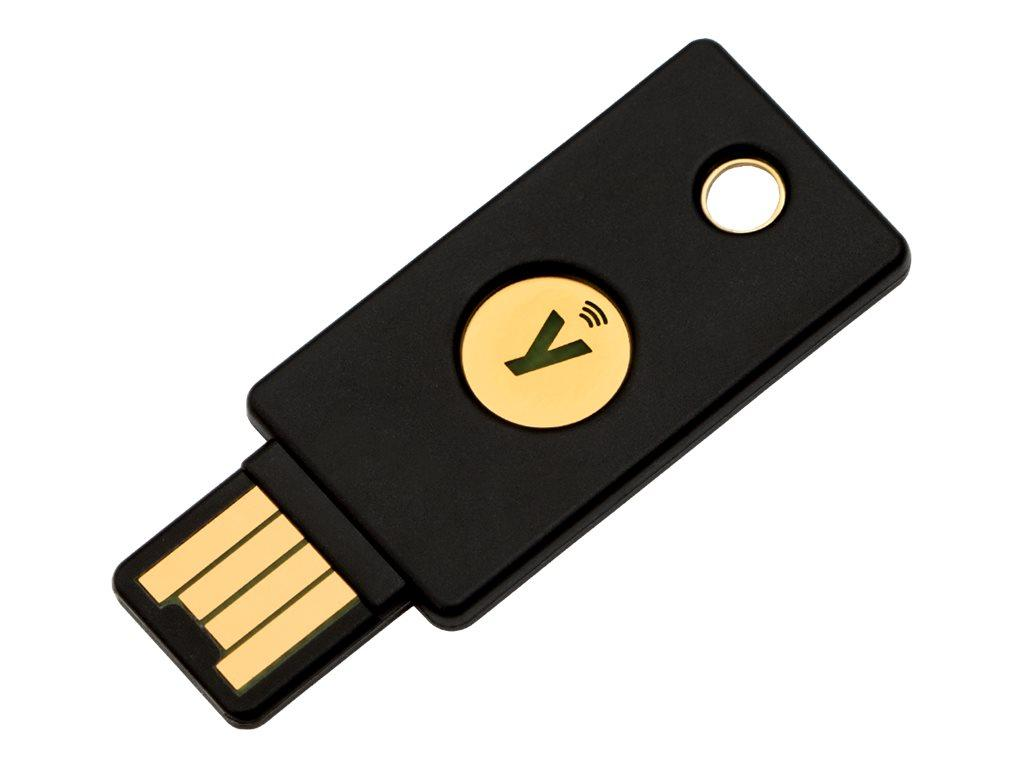
\includegraphics[width=0.3\textwidth]{img/abbildungen/yubikey.jpeg}
	\captionsetup{format=hang}
	\caption{Umsetzungsmöglichkeit mit Keycloak}
\end{figure}

 \begin{itemize}
    \item Ein Security Key ist eine Hardware, welche es ermöglicht einen Nutzer zu authentifizieren, indem dieser mit dem Security Key interagiert (beispielsweise durch einen Knopfdruck) \cite{reynolds2018tale}.
    \item Häufig werden Security Keys so designed, dass sie per USB an einen Computer angeschlossen werden können \cite{reynolds2018tale}.
    \item Die YubiKeys 5 ermöglichen drei Arten der Authentifizierung:
    1. \ac{SFA} Ersetzt Passwörter durch ein passwortloses \textit{tap-n-go} Verfahren.
    2. \ac{2FA} Sichert ein Passwort zusätzlich mit einem \textit{tap-n-go} Faktor ab. Der Security ist somit der zweite Faktor (\textit{something you have}).
    3. \ac{MFA} Verbindet die passwortlose \textit{tap-n-go} Authentifizierung mit einer PIN. (EIG AUCH SFA ODER NICHT)
 \end{itemize}

\subsection{Usability}

\begin{itemize}
    \item Vorteile:
    \item Ergebnisse zeigen, dass Nutzer grundsätzlich bereit sind, Passwörter durch passwortlose Verfahren zu ersetzen \cite{lyastani2020fido2}.
    \item Passwortlose Verfahren mit Yubikey wurden mehr akzeptiert als tradionelle passwortbasierte Verfahren \cite{lyastani2020fido2}.
    \item Implizite Garantie, dass sich lediglich Nutzer authentifizieren können, welche auch im Besitz des Authentifizierungsgerätes sind. \cite{lyastani2020fido2}.
    \item Durch die Nutzung von FIDO2 kann die Usability verbessert werden, da Nutzer sich keine Passwörter mehr merken müssen. Häufig wird das Verwalten der immer höher werdenden Anzahl an Passwörtern als Problem angesehen \cite{lyastani2020fido2} \cite{farke2020you}.
    \item Es wird ein deutlich geringerer kognitiver Aufwand benötigt, da Nutzer keine neuen Passwörter mehr erstellen und merken müssen \cite{lyastani2020fido2}.
    \item Zum aktuellen Zeitpunkt wird FIDO2 bereits von einer Vielzahl an Browsern unterstützt. Zusätzlich bieten immer mehr Online-Dienste die Möglichkeit an sich mit Hilfe von FIDO2 zu authentifizieren \cite{lyastani2020fido2} \cite{farke2020you}.
    \item Es handelt sich um offene und standardisierte Protokolle \cite{farke2020you}.
    \item Nachteile:
    \item Im Falle einer \ac{SFA} wird der Verlust des Authentifizierungsgerätes als größtes Problem angesehen. Bei Verlust hat auch der Nutzer keinen Zugriff mehr und aktuell gibt es noch keine sichere und effiziente Möglichkeiten, um den Zugriff wiederherzustellen (vor allem ohne Pause) \cite{lyastani2020fido2}.
    \item Da es sich um zusätzliche Hardware handelt kann diese ebenfalls kaputt gehen \cite{farke2020you}.
    \item Im Unternehmenskontext, kann die Verwaltung und Verteilung der Authentifizierungsgeräte zu einem Problem werden \cite{farke2020you}. 
    \item Da es sich um Hardware handelt, können Zugänge nicht an vertraute Personen weitergegeben werden, da der Zugang nur mit dem Authentifizierungsgerät möglich ist \cite{lyastani2020fido2}.
    \item Ohne das Authentifizierungsgerät sind keine spontanen Logins möglich \cite{lyastani2020fido2}.
    \item Es wird ein physischer Aufwand benötigt, da das Authentifizierungsgerät mitgeführt werden muss \cite{lyastani2020fido2}.
    \item Bereits das aus der Tasche holen des Authentifizierungsgerätes ist für manche Nutzer bereits eine Hürde \cite{farke2020you}.
    \item Authentifizierungsgeräte sind häufig mit Kosten verbunden, welche vom Nutzer getragen werden müssen \cite{lyastani2020fido2}.
    \item Nutzer haben Probleme ein neues Verfahren für die Authentifizierung zu nutzen, da sie sich an das alte Verfahren gewöhnt haben. Das führt dazu, dass Nutzer das neue Verfahren als kompliziert und ungewohnt empfinden. Sie verfügen häufig nicht über das nötige Wissen, um die Funktion und Sicherheit des Verafahrens zu verstehen \cite{lyastani2020fido2}.
    \item Selbst Nutzern, welchen das Konzept der passwortlosen Authentifizierung gefällt, nutzen häufig weiterhin Passwörter \cite{farke2020you}.
    \item Nutzer wollen keine Angewohnheiten verändern, wenn die nicht dazu gezwungen sind \cite{farke2020you}.
    \item Nutzer verwenden lieber Passwörter, da sie das Konzept und die Technologie besser verstehen \cite{lyastani2020fido2}.
    \item Nicht zwangsweise schneller als die Nutzung von Passwortmanagern \cite{farke2020you}.
    \item Allgemein fällt das Feeback von Nutzern weniger positiv aus, wenn diese vorher bereits Passwortmanager genutzt haben \cite{farke2020you}.
    \item Fazit:
    \item Insgesamt lassen sich noch nicht alle Szenarien mit FIDO2 abdecken. Es gibt noch spezielle Fälle, in welchen die Nutzung von Passwörtern weiterhin notwendig ist \cite{lyastani2020fido2}.
    \item 
\end{itemize}

\section{Fido2}

\begin{figure}[h]
	\centering 
	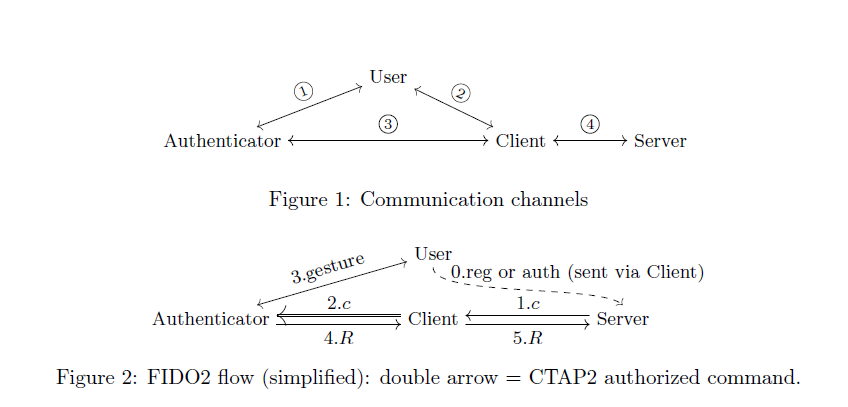
\includegraphics[width=1\textwidth]{img/abbildungen/fido2-simple.png}
	\captionsetup{format=hang}
	\caption{Umsetzungsmöglichkeit mit Keycloak}
\end{figure}

\begin{figure}[h]
	\centering 
	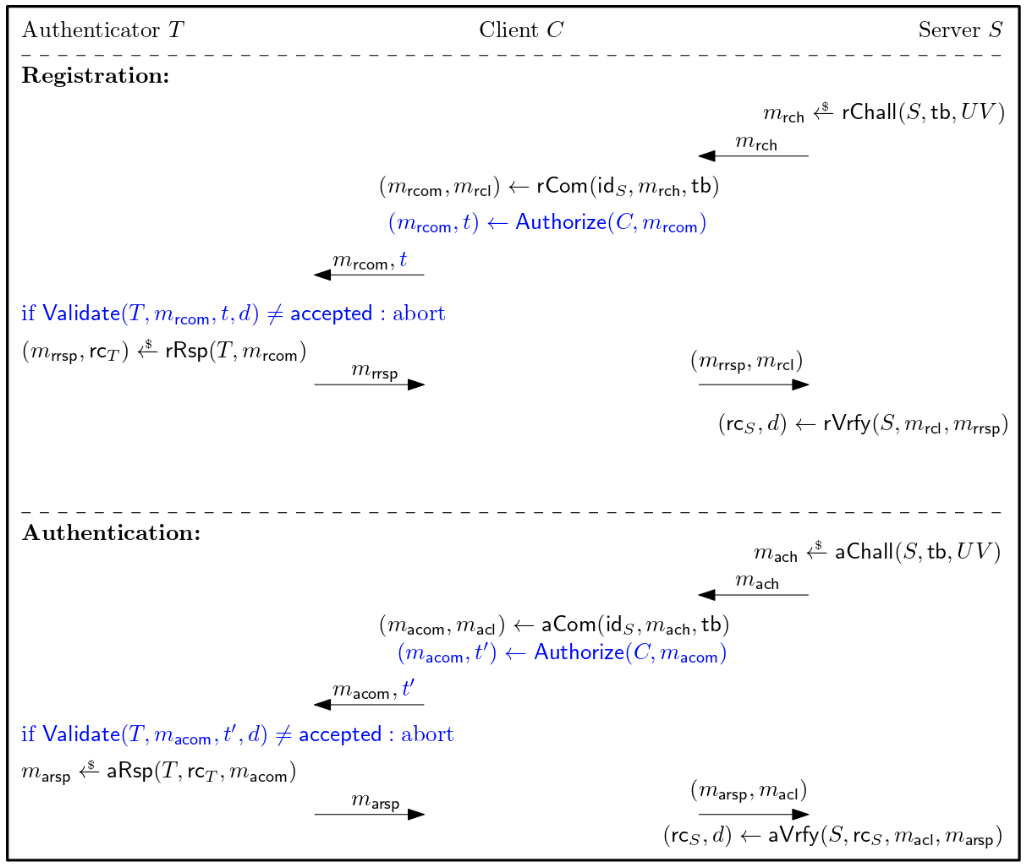
\includegraphics[width=1\textwidth]{img/abbildungen/Fido2.png}
	\captionsetup{format=hang}
	\caption{Umsetzungsmöglichkeit mit Keycloak}
\end{figure}

\begin{figure}[h]
	\centering 
	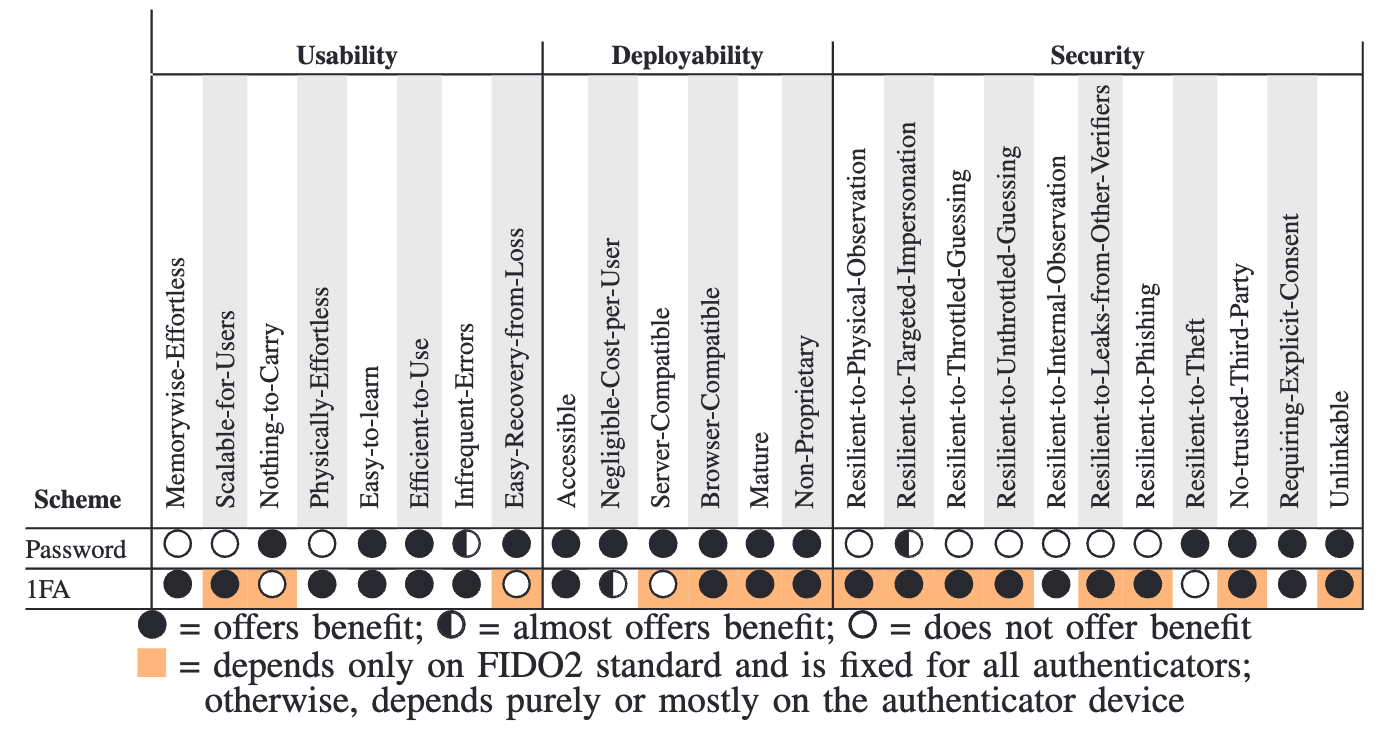
\includegraphics[width=1\textwidth]{img/abbildungen/fido2_usability.png}
	\captionsetup{format=hang}
	\caption{Umsetzungsmöglichkeit mit Keycloak}
\end{figure}

\begin{itemize}
    \item FIDO2 wird von der \ac{FIDO} und dem \ac{W3C} entwickelt und bereitgestellt \cite{lyastani2020fido2} \cite{farke2020you}.
    \item Die \ac{FIDO} Allianz ist eine Organisation mit weltweit über 250 Mitgliedern. Darunter befinden sich Unternehmen wie Google, Microsoft, Apple Amazon, Facebook, Visa und viele mehr \cite{lyastani2020fido2} \cite{farke2020you}.
    \item Ziel ist es Nutzer zu authentifizieren, ohne, dass diese eine Passwort nutzen müssen \cite{morii2017research} \cite{barbosa2021provable}.
    \item Basiert auf der Nutzung eines internen oder externen Authentifizierungsgerätes \cite{morii2017research} \cite{barbosa2021provable}.
    \item Dabei können Authentifizierungsgeräte, ebenfalls mit einer PIN oder einem biometrischen Merkmal, geschützt werden \cite{farke2020you}.
    \item Hierbei ist ein PIN allerdings nicht gleichzusetzen mit einem Passwort. Der PIN wird lediglich für das Authentifizierungsgerät genutzt und wird auch nur auf diesem gespeichert \cite{farke2020you} \cite{barbosa2021provable}.
    \item Es handelt sich dabei also auch nicht um eine \ac{MFA}, sondern, um einen einzelnen Faktor, welcher lediglich den Zugriff das Gerät selbst authentifiziert \cite{barbosa2021provable}.
    \item FIDO2 unterstützt sowohl \ac{MFA} als auch \ac{SFA} \cite{lyastani2020fido2} \cite{farke2020you}.
    \item Viele Alternativen zur passwortbasierten AUthentifizierung existieren bereits. Diese werden allerdings nur in einem sehr geringen Ausmaß genutzt \cite{farke2020you}.
    \item Stellt Zugangsdaten bereit, welche nicht gephisht oder von Datenlecks betroffen sein können \cite{lyastani2020fido2}.
    \item Das liegt daran, dass keine geteilten Geheimnisse zwischen Nutzer und Dienst existieren, welche auf einem Server gespeichert werden \cite{morii2017research}.
    \item Wird von fast allen Browsern standardmäßig unterstützt \cite{lyastani2020fido2}.
    \item Viele verfügbare Authentifizierungsgeräte. Z.B. Security Keys oder auch Smartphones. Beispielsweise Apples Touch ID oder Face ID \cite{lyastani2020fido2}.
    \item Besteht aus zwei Komponenten: CTAP2 für die Kommunikation zwischen Client und Authentifizierungsgerät und WebAuthn für die Kommunikation zwischen Client und Server \cite{farke2020you}.
    \item Dabei wird WebAuthn von der \ac{W3C} spezifiziert und CTAP2 von der \ac{FIDO} Allianz \cite{farke2020you}.
\end{itemize}

\subsection{Webauthn}

\begin{itemize}
    \item WebAuthn ist ein Standard, welcher von dem \ac{W3C} entwickelt wird. Das Protokoll erlaubt es Webanwendungen Nutzer zu authentifizieren. Dies kann dabei auch über \ac{CTAP2} erfolgen \cite{lyastani2020fido2}. ?
    \item Wurde 2019 ein offizieller Webstandard \cite{farke2020you}.
    \item Spezifiziert eine standardiserte, vom Browser unabhängige JavaScript API zur Authentifizierung von Nutzern für Webanwendungen. So können Webanwendungen eine Authentifizierung integrieren, welche resistent gegenüber Phishing, Datenlecks und Passwortdiebstahl ist. Anstelle von geteilten Geheimnissen nutzt WebAuthn public-key Kryptographie, um einzigartige Zugangsdaten für jede Webanwendung zu erstellen, welche nur auf dem Gerät des Nutzers gespeichert werden \cite{farke2020you}.
    \item Passwortloses Challenge-Response-Verfahren zwischen Client und Server \cite{barbosa2021provable}.
    \item WebAuthn unterstützt zwei Opertationen: Registrierung und Anmeldung \cite{barbosa2021provable}.
    \item In der Registrierungsphase sendet der Server dem Authentifizierungsgerät über den CLient eine zufällige Challenge. In dieser Phase signiert das Authentifizierungsgerät mit Hilfe seines privaten Schlüssels die CHallenge und sendet zusätzlich  öffentliche Anmeldedaten für zukünftige Anmeldungen an den Server. Meldet sich ein bereits registrierter Nutzer an, wird die Challenge des Servers erneut von dem Authentifizierungsgerät signiert zurück an den Server gesendet. Der Server kann die Signatur mit Hilfe des öffentlichen Schlüssels verifizieren und den Nutzer authentifizieren \cite{barbosa2021provable}.
    \item Registrierungsphase:
    Der Server \textit{S} sendet eine challenge message $m_{rch}$ über den Client \textit{C} an den Security Key. Diese Challenge beinhaltet eine randomisierte Nonce, Parameter (beispielsweise, ob eine Nutzerverifizierung notwendig ist) und optional einen wert \textit{tb}, welcher den zugrunde liegenden Kanal eindeutig identifiziert (typischerweise eine \ac{TLS} Verbindung). Der Client \textit{C} erhält die challenge message $m_{rch}$ und wandelt diese in eine command message $m_{rcom}$ und eine client mesasage $m_{rcl}$ um. die command message $m_{rcom}$ wird an den Security Key $T$ übermittelt. Der Security Key $T$ erzeugt öffentlich-privates Schlüsselpaar, welches an den Server $S$ gebunden ist und diesem ermöglicht eine Verifizierung, während der folgenden AUthentifizierungsphase durchzuführen. Zudem gibt der Security Key $T$ eine response message $m_{rrsp}$ aus. Der Client übergibt diese und die client message $m_{rcl}$ an den Server $S$. Die response message $m_{rrsp}$ beinhaltet einen \textit{attestation type}, welcher es dem Server $S$ ermöglicht eine Verifizierung während der Registrierungsphase durchzuführen und beinhaltet den öffentlichen Schlüssel. WebAuthN 2 unterstützt fünf \textit{attestation types}. Häufig werden die types \textit{None} und \textit{Basic} verwendet. Die restlichen types sind \textit{Self}, \textit{AttCA} und \textit{AnonCA}. \cite{bindel2022fido2}
    \item Authentifizierungsphase:
    Der Client empfängt die challenge message $m_{ach}$ von Server $S$ und wandelt diese in eine command message $m_{acom}$ und eine client message $m_{acl}$ um. Die command message $m_{acom}$ wird an den Security Key $T$ übermittelt. Der Security Key $T$ erzeugt eine response message $m_{arsp}$, welche mit dem privaten Schlüssel signiert wird und sendet diese an den Server $S$ (über den Client $C$). Der Server $S$ akzeptiert die response message $m_{arsp}$ und die client message $m_{acl}$ nur, wenn sie sich mit dem dazugehörigen öffentlichen Schlüssel verifizieren lassen. \cite{bindel2022fido2}
    \item Die Sicherheit von WebAuthn basiert auf dem Beweis, dass RSASSA PKCS1-v1\_5 und RSASSA-PSS als \ac{EUF-CMA} gelten und der Annahme, dass SHA-256 kollisionsresistent ist \cite{barbosa2021provable}.
\end{itemize}

\subsection{CTAP2}
\begin{itemize}
    \item 2018 wurde \ac{CTAP2} als internationaler Standard der \ac{ITU-T} anerkannt \cite{barbosa2021provable}.
    \item \ac{CTAP2} ist ein Protokoll auf der Anwendungsebene, welches für die Kommunikation zwischen eines WebAuthn Clients und eines konformen Authentifizierungsgerätes genutzt wird. Das Authentifizierungsgerät kann dabei ein externes Gerät sein wie beispielsweise ein Security Key, welches über USB, Bluetooth oder NFC eine Verbindung mit dem Client aufbaut. Aber auch ein internes Gerät wie beispielsweise ein Fingerabdruckscanner oder ein Trusted Platform Module können als Authentifizierungsgerät genutzt werden \cite{lyastani2020fido2}.
    \item \ac{CTAP2} spezifiziert, die Kommunikation zwischen einem Authentifizierungsgerät und einem Client. Der Client ist dabei üblicherweise ein Webbrowser. Das Ziel ist es zu garantieren, dass der CLient das AUthentifizierungsgerät nur nutzen darf, wenn der Nutzer dies erlaubt. Dafür muss der Nutzer beispielsweise einen Knopf am Authentifizierungsgerät drücken und/oder sich mit Hilfe eines PINs oder eines biometrischen Merkmals beim AUthentifizierungsgerät authentifizieren \cite{barbosa2021provable}.
    \item Das Ziel ist es somit einen Client an das AUthentifizierungsgerät zu binden. Ist ein CLient nicht an das authentifizerungsgerät gebunden, kann dieser sich nicht authentifizieren \cite{barbosa2021provable}.
    \item besteht aus mehreren Phasen. 
    1. In der Setup Phase initialisiert ein Client $C'$ einen PIN, welcher vom User übergeben wird an den Security Key $T$.
    2. In der Binding Phase tauschen ein Client $C$ (nicht zwangsweise $C'$) und der Security Key $T$ einen gemeinsamen Verbindungsstatus aus, wenn der Client $C$ in der Lage ist, Informationen über die auf dem Security Key $T$ gespeicherte PIN zu liefern. So soll eine einzigartige Verbindung zwischen dem Client $C$ und dem Security Key $T$ hergestellt werden. Schlägt der Client $C$ drei mal in Folge fehl die PIN zu liefern, wird der Security Key $T$ neu gestartet und der Verbindungsstatus wird zurückgesetzt. Schlägt der Client $C$ insgesamt acht mal fehl, wird der Security Key $T$ gesperrt.
    3. Ist diese Phase erfolgreich, autorisiert der Client $C$ jeden Befehl, indem eer einen Tag $t$ ausgibt, welcher mit der command message an den Security Key $T$ übermittelt wird. Der Security Key $T$ fährt lediglich fort, wenn eine \textit{positive decision} $d$ des Users vorliegt (beispielsweise einem Knopfdruck) und validiert darauf hin die command message und den Tag $t$. \cite{bindel2022fido2}
    \item \ac{CTAP2} nutzt unauthentifizierten Diffie-Hellman Schlüsselaustausch \cite{barbosa2021provable}.
    \item Dieser kann von \ac{MITM} Angriffen betroffen sein \cite{barbosa2021provable}.
    \item In der Binding Phase sendet das Authentifizierungsgerät dem CLient ein pinToken, welcher beim hochfahren des Authentifizierungsgerätes generiert wird. Dieser pinToken wird lokal auf dem AUthentifizierungsgerät gespeichert und wird von dem verbundenen Client in der Access Channel Phase genutzt, um die nachfolgenden Nachrichten des Clients zu autorisieren \cite{barbosa2021provable}.
    \item Jedem AUthentifizierungsgerät wird ein pinToken pro hochfahren zugeordnet. Das bedeutet mehrere CLients erezugen mehrere Access Channels mit dem selbem Authentifizierungsgerät und dem selben pinToken \cite{barbosa2021provable}.
    \item Dadurch wird die Sicherheit von \ac{CTAP2} limitiert ??
\end{itemize}

\subsubsection{CTAP2.1}
\begin{itemize}
    \item Gilt in Verbindung mit WebAuthn 2 als \ac{PQ} bereit, da ein Operationsmodus ermöglicht wird, der nur kryptographische Primitive, digitale Signaturen und \ac{KEM} verwendet \cite{bindel2022fido2}.
    \item Im Gegensatz zu \ac{CTAP2} basiert CTAP2.1 nicht auf unauthentifizierten Diffie-Hellman Schlüsselaustausch, sondern auf einem sogeannten \ac{puvProtocol}, wodurch die \ac{PQ}-Sicherheit ermöglicht wird \cite{bindel2022fido2}.
    \item In \ac{CTAP2} wird der Verbindungszustand als \textit{pinToken} definiert, welcher aus mehreren 128 Bit-Blöcken besteht und keine maximale Begrenzung der Länge beseitzt. In CTAP2.1 wird der Verbindungszustand als \textit{pinUvAuthToken} definiert welcher eine feste Länge von 128 oder 256 Bit besitzt \cite{bindel2022fido2}.
    \item Der pinToken von \ac{CTAP2} wird bis zum nächsten Neustart wiederverwendet. Der pinUvAuthToken von CTAP2.1 wird nach jeder erfolgreichen Authentifizierung neu generiert. Das führt dazu, dass CTAP2.1 eine \ac{SUF}-t' Sicherheit aufweist und \ac{CTAP2} lediglich eine \ac{UF}-t' Sicherheit \cite{bindel2022fido2}.
    \item \ac{CTAP2} erlaubt es Security Keys und Clients nur den pinUvAuthToken zu teilen, wenn der Nutzer den korrekten PIN eingegeben hat. CTAP2.1 ermöglicht zusätzlich, dass der Nutzer sich mit Hilfe eines biometrischen Merkmals authentifiziert \cite{bindel2022fido2}.
\end{itemize}

\subsection{Sicherheit}

\begin{itemize}
    \item FIDO2 ist eine Erweiterung des FIDO U2F Protokolls und bietet die selbe Sicherheit wie public key Kryptographie \cite{lyastani2020fido2}.
    \item Es handelt sich um geprüfte assymetrische Kryptographie \cite{farke2020you}.
    \item Es handelt sich dabei um ein Challenge-Response-Verfahren mittels Hardware basierten Authentifizierungsgeräten. Dies bietet einige Vorteile gegenüber passwortbasierten Verfahren. Es gibt keine geteilten Geheimnisse zwischen Usern und Diensten, welche durch Phishing oder Datenlecks kompromittiert werden können. Dabei ist das selbe Authentifizierungsgerät für mehrere Dienste nutzbar, ohne, dass sich dabei eine Verknüpfung zurückführen lässt \cite{lyastani2020fido2} \cite{farke2020you}.
    \item lediglich die Session kann kompromittiert werden \cite{morii2017research}.
    \item Authentifizierungsgeräte lassen sich mit zusätzlichen PINs oder biometrischen Merkmalen absichern, um sich ebenfalls vor Diebstahl schützen \cite{barbosa2021provable}.
    \item Unauthentifizierter Diffie-Hellman Schlüsselaustausch könnte durch ein \ac{PAKE} Verfahren ersetzt werden \cite{barbosa2021provable}.
    \item Das Paper gibt an, dass dieses sicherer und effizienter sein soll \cite{barbosa2021provable}.
    \item In folgendem Szenario: 1. Der Nutzer besitzt einen Security Key, welcher mit einem drückbaren Knopf oder ähnlichen ausgestattet ist. 2. Der Security Key ist mit einem geheimen PIN geschützt. 3. Der Nutzer autorisiert vertrauten Clients auf den Security Key zuzugreifen. 4. Der Nutzer verbindet seinen Security Key mit mehreren Clients und nutzt diese um sich bei mehreren Webdiensten zu registrieren/anzumelden.
    Dann ist versichert, dass:
    1. Die Authentifizierung von dem Security Key durchgeführt wurde, welcher die genutzen Zugangsdaten bei dem Webdienst registriert hat.
    2. ein autorisierter Befehl auf den Security Key zugegriffen hat.
    3. und dieser autorisierte Befehl von einem autorisierten Client beauftragt wurde (sollte der Nutzer den korrekten PIN eingegeben haben).
    Dies setzt voraus, dass:
    1. Der Security Key nicht gestohlen wurde.
    2. Der PIN des Security Keys nicht kompromittiert wurde.
    3. Der autorisierte Client nicht kompromittiert wurde (korrekte Ausführung von \ac{CTAP2} und CLient ist nicht von böswilliger Software betroffen).
    \cite{barbosa2021provable}.
    \item Wird ein Security Key gestohlen, kann dieser nur genutzt werden, wenn ebenfalls der PIN bekannt ist \cite{barbosa2021provable}.
\end{itemize}
